\documentclass[a4paper, 12pt]{article} 

%--------------------------------------
%Russian-specific packages
%--------------------------------------
%\usepackage[warn]{mathtext}
\usepackage[T2A]{fontenc}
\usepackage[utf8]{inputenc}
\usepackage[english,russian]{babel}
\usepackage[intlimits]{amsmath}
\usepackage{esint}
%--------------------------------------
%Hyphenation rules
%--------------------------------------
\usepackage{hyphenat}
\hyphenation{ма-те-ма-ти-ка вос-ста-нав-ли-вать}
%--------------------------------------
%Packages
%--------------------------------------
\usepackage{amsmath}
\usepackage{amssymb}
\usepackage{amsfonts}
\usepackage{amsthm}
\usepackage{latexsym}
\usepackage{mathtools}
\usepackage{epstopdf}
\usepackage{etoolbox}%Булевые операторы
\usepackage{extsizes}%Выставление произвольного шрифта в \documentclass
\usepackage{geometry}%Разметка листа
\usepackage{indentfirst}
\usepackage{wrapfig}%Создание обтекаемых текстом объектов
\usepackage{fancyhdr}%Создание колонтитулов
\usepackage{setspace}%Настройка интерлиньяжа
\usepackage{lastpage}%Вывод номера последней страницы в документе, \lastpage
\usepackage{soul}%Изменение параметров начертания
\usepackage{hyperref}%Две строчки с настройкой гиперссылок внутри получаеммого
\usepackage[usenames,dvipsnames,svgnames,table,rgb]{xcolor}% pdf-документа
\usepackage{multicol}%Позволяет писать текст в несколько колонок
\usepackage{cite}%Работа с библиографией
\usepackage{subfigure}% Человеческая вставка нескольких картинок
\usepackage{tikz}%Рисование рисунков
\usepackage{float}
% Для картинок Моти
\usepackage{misccorr}
\usepackage{lscape}
\usepackage{cmap}
\usepackage{hyperref}
\usepackage{xcolor}



\usepackage{graphicx,xcolor}
\graphicspath{{Pictures/}}
\DeclareGraphicsExtensions{.pdf,.png,.jpg}

%----------------------------------------
%Список окружений
%----------------------------------------
\newenvironment {theor}[2]
{\smallskip \par \textbf{#1.} \textit{#2}  \par $\blacktriangleleft$}
{\flushright{$\blacktriangleright$} \medskip \par} %лемма/теорема с доказательством
\newenvironment {proofn}
{\par $\blacktriangleleft$}
{$\blacktriangleright$ \par} %доказательство
%----------------------------------------
%Список команд
%----------------------------------------
\newcommand{\grad}
{\mathop{\mathrm{grad}}\nolimits} %градиент

\newcommand{\diver}
{\mathop{\mathrm{div}}\nolimits} %дивергенция

\newcommand{\Def}[1]
{\underline{\textbf{#1}}} %определение

\newcommand{\RN}[1]
{\MakeUppercase{\romannumeral #1}} %римские цифры

\newcommand {\theornp}[2]
{\textbf{#1.} \textit{ #2} \par} %Написание леммы/теоремы без доказательства

\newcommand{\qrq}
{\ensuremath{\quad \Rightarrow \quad}} %Человеческий знак следствия

\newcommand{\qlrq}
{\ensuremath{\quad \Leftrightarrow \quad}} %Человеческий знак равносильности

\renewcommand{\phi}{\varphi} %Нормальный знак фи

\newcommand{\me}
{\ensuremath{\mathbb{E}}}

\newcommand{\md}
{\ensuremath{\mathbb{D}}}




%\renewcommand{\vec}{\overline}




%----------------------------------------
%Разметка листа
%----------------------------------------
\geometry{top = 3cm}
\geometry{bottom = 2cm}
\geometry{left = 1.5cm}
\geometry{right = 1.5cm}
%----------------------------------------
%Колонтитулы
%----------------------------------------
\pagestyle{fancy}%Создание колонтитулов
\fancyhead{}
%\fancyfoot{}
\fancyhead[R]{\textsc{ОДУ: Контрольная работа 2}}%Вставить колонтитул сюда
%----------------------------------------
%Интерлиньяж (расстояния между строчками)
%----------------------------------------
%\onehalfspacing -- интерлиньяж 1.5
%\doublespacing -- интерлиньяж 2
%----------------------------------------
%Настройка гиперссылок
%----------------------------------------
\hypersetup{				% Гиперссылки
	unicode=true,           % русские буквы в раздела PDF
	pdftitle={Заголовок},   % Заголовок
	pdfauthor={Автор},      % Автор
	pdfsubject={Тема},      % Тема
	pdfcreator={Создатель}, % Создатель
	pdfproducer={Производитель}, % Производитель
	pdfkeywords={keyword1} {key2} {key3}, % Ключевые слова
	colorlinks=true,       	% false: ссылки в рамках; true: цветные ссылки
	linkcolor=blue,          % внутренние ссылки
	citecolor=blue,        % на библиографию
	filecolor=magenta,      % на файлы
	urlcolor=cyan           % на URL
}
%----------------------------------------
%Работа с библиографией 
%----------------------------------------
\renewcommand{\refname}{Список литературы}%Изменение названия списка литературы для article
%\renewcommand{\bibname}{Список литературы}%Изменение названия списка литературы для book и report
%----------------------------------------
\begin{document}
\begin{titlepage}
\begin{center}


\vfill






\textbf{РЕШЕНИЯ ЗАДАЧ \\[3mm]
КОНТРОЛЬНОЙ РАБОТЫ №2\\[3mm]
по курсу "Обыкновенные дифференциальные уравнения"
\\[20mm]
}
\end{center}

\texttt{Исходный код:} \href{https://github.com/pholeque/ode/tree/main/test2-solutions}{\color{red} {https://github.com/pholeque/ode/tree/main/test2-solutions}}
\tableofcontents

\end{titlepage}

\newpage




	\section{Вариант IA}
		\subsection {Задача 1}


 Решить систему дифференциальных уравнений (Задача Коши): 
\begin{equation}
\left\{
\begin{array}{lr}
\dot{x} = 3x-2y\\
\dot{y} = 2x-2y
\end{array}
\right.
, \;\;\;\; x(\cdot)\in \textbf{R},\; y(\cdot)\in \textbf{R}
\label{eq:1}
\end{equation}

\textbf{Решение:} \par
Обозначим 
\[
A = \left(
\begin{array}{cc}
-3 & -2\\
2 & -2\\
\end{array}
\right)\]

(i) Стационарные точки:

\[
\left\{
\begin{array}{lr}
\dot{x} = 0\\
\dot{y} = 0
\end{array}
\right.
\Leftrightarrow (0;0)
\]


(ii) Найдем собственные числа матрицы A:
\[det(A-\lambda \hat{I})=
\begin{vmatrix}
3-\lambda & -2 \\
2 & -2-\lambda
\end{vmatrix}
=0\]

\[\lambda_1=-1, \; \lambda_2=2\]
\\Найдем собственные векторы:
\[\lambda_1=-1,\;\;\;\;\; p^1=
\left(
\begin{array}{cc}
1\\
2\\
\end{array}
\right)
\]



\[\lambda_1=2,\;\;\;\; p^2=
\left(
\begin{array}{cc}
2\\
1\\
\end{array}
\right)
\]
Каноническое преобразование координат:
\[A = S\Lambda S^{-1}\]
\[
S = \left(
\begin{array}{cc}
1 & 2\\
2 & 1\\
\end{array}
\right)\;\;\;\;\;
S^{-1} = \left(
\begin{array}{cc}
-1 & 2\\
2 & -1\\
\end{array}\right)\;\;\;\;\;
\Lambda = \left(
\begin{array}{cc}
-1 & 0\\
0 & 2\\
\end{array}\right)
\]

Система в новых координатах:
\[\left(
\begin{array}{c}
\dot{\alpha}_1\\
\dot{\alpha}_2
\end{array}
\right)=\Lambda\left(
\begin{array}{c}
{\alpha}_1 \\
{\alpha}_2
\end{array}
\right)\]


(iii) Прямые, при пересечении которых фазовые траектории параллельны осям $x$ и $y$.\\
Параллельно оси y:
\[\dot{x} = 3x-2y=0\Leftrightarrow y = 3/2x\]\\
Параллельно оси x:
\[\dot{y} = 2x-2y=0\Leftrightarrow y = x\]
\begin{figure}[H]
	\centering
	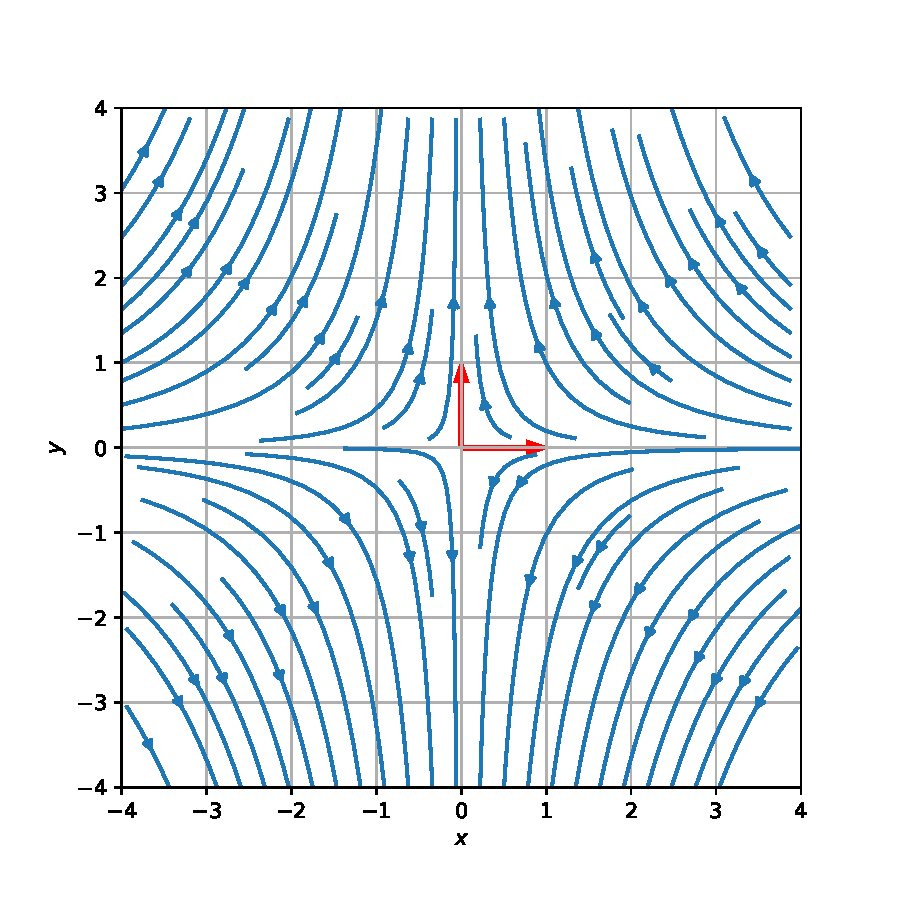
\includegraphics[scale=0.7]{1a1_0}
	\caption{Фазовый портрет в канонических координатах}
	\label{im:1a1_0}
\end{figure}



(iv) Фазовый портрет(\ref{eq:1}) в исходных координатах:

\begin{figure}[H]
	\centering
	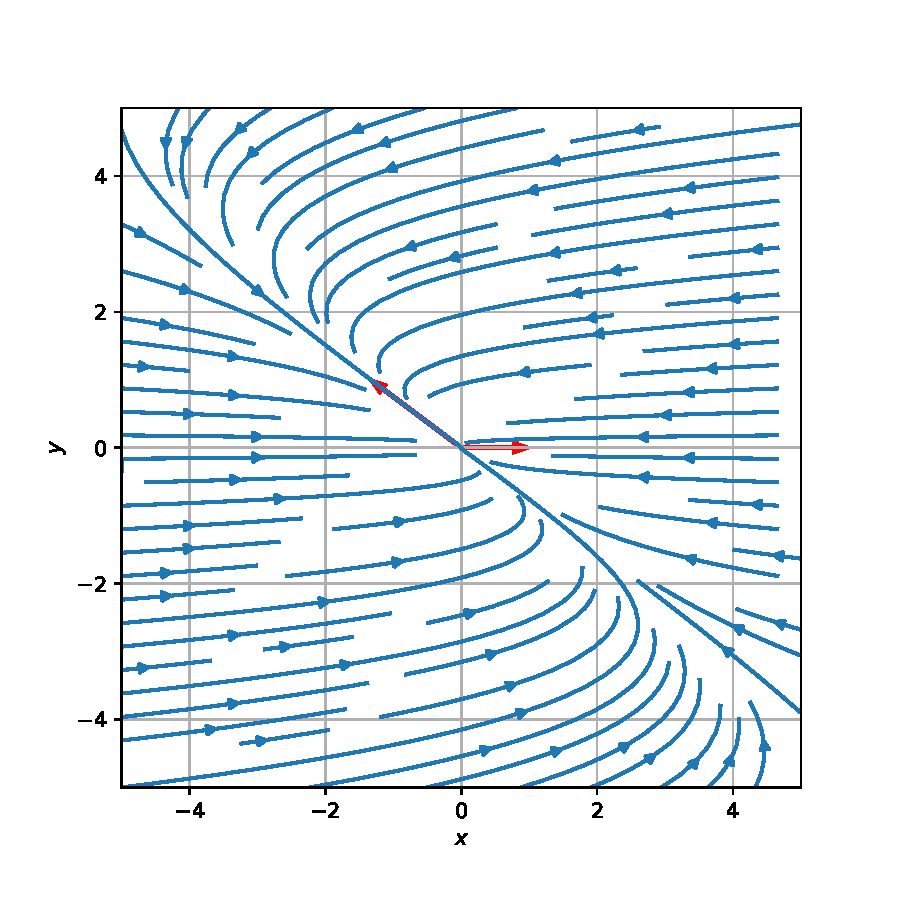
\includegraphics[scale=0.7]{1a1_1}
	\caption{Фазовый портрет в исходных координатах}
	\label{im:1a1_1}
\end{figure}

(v) $\lambda_{1,2}$ разных знаков, картина -- \textbf{седловая точка}.







	\subsection {Задача 2}
 Решить систему дифференциальных уравнений (Задача Коши): 
\begin{equation}
\left\{
\begin{array}{lr}
\dot{x} = -x+4y+2e^{3t}\\
\dot{y} = -x+3y-2
\end{array}
\right.
, \;\;\;\; x(\cdot)\in \textbf{R},\; y(\cdot)\in \textbf{R}
\label{eq:2}
\end{equation}

\textbf{Решение:} \par
Обозначим 
\[
A = \left(
\begin{array}{cc}
-1 & 4\\
-1 & 3\\
\end{array}
\right)\]

(i) Найти общее решение соответствующей однородной системы.
\[det(A-\lambda \hat{I})=
\begin{vmatrix}
-1-\lambda & 4 \\
-1 & 3-\lambda
\end{vmatrix}
=0\]


\[\lambda =1\;\;\text{-- собственное число кратности 2}\]
Собственный вектор:
\[p=
\left(
\begin{array}{cc}
2\\
1\\
\end{array}
\right)
\]
Пространство векторов имеет размерность 1:
\[\dim \{ p\in \textbf {R}^2: p_1^1=-p_2^1\}=1\]
Собственному числу соответствует одномерное пространство собственных векторов. Найдем присоединенный вектор:\\
\[(A-\lambda \hat{I})v=p\]

\[v=
\left(
\begin{array}{cc}
-1\\
0\\
\end{array}
\right)
\]
Каноническое преобразование координат:
\[A = S\Lambda S^{-1}\]
\[
S = \left(
\begin{array}{cc}
2 & -1\\
1 & 0\\
\end{array}
\right)\;\;\;\;\;
S^{-1} = \left(
\begin{array}{cc}
0 & 1\\
-1 & 2\\
\end{array}\right)\;\;\;\;\;
\Lambda = \left(
\begin{array}{cc}
1 & 1\\
0 & 1\\
\end{array}\right)
\]
Получаем общее решение однородной системы:
\[\left(
\begin{array}{c}
x(t)\\
y(t)
\end{array}
\right)=e^{At}\left(
\begin{array}{c}
C_1 \\
C_2
\end{array}
\right)=Se^{\Lambda}S^{-1}\left(
\begin{array}{c}
C_1 \\
C_2
\end{array}
\right)=e^t
\left(
\begin{array}{cc}
2 & -1 \\
1 & 0
\end{array}
\right)
\left(
\begin{array}{cc}
1 & t \\
0 & 1
\end{array}
\right)
\left(
\begin{array}{cc}
0 & 1 \\
1- & 2
\end{array}
\right)\left(
\begin{array}{c}
C_1 \\
C_2
\end{array}
\right)=\]\[
=e^t
\left(
\begin{array}{cc}
1-2t & 4t \\
-t & 1+2t
\end{array}
\right)\left(
\begin{array}{c}
C_1 \\
C_2
\end{array}
\right)\]
Частное решение будем искать методом неопределенных коэффициентов:
\[x(t)_{\text{частн}}=ae^{3t}+b\]
\[y(t)_{\text{частн}}=ce^{3t}+d\]
Подставляя эти выражения в систему (\ref{eq:2}), получим:
\[
\left\{
\begin{array}{lr}
3ae^{3t}=-(ae^{3t}+b)+4(ce^{3t}+d)+2e^{3t}\\
3ce^{3t}=-(ae^{3t}+b)+3(ce^{3t}+d)-2\\
\end{array}
\right.
\]
Отсюда находим:
\[
\left\{
\begin{array}{lr}
a = 0\\
c = - \frac 1 2 \\
d = -2 \\
b=-8
\end{array}
\right.
\]
Общее решение уравнения есть сумма частного и однородного:

\begin{equation}
x(t) = e^t\left(\left(1-2t\right)C_1+4tC_2\right)-8
\label{eq:3}
\end{equation}
\begin{equation}
y(t) = e^t\left(-tC_1+\left(2t+1\right)C_2\right)-\frac 1 2 e^{3t}-2
\label{eq:4}
\end{equation}

(ii) Найти траекторию системы (\ref{eq:2}), проходящую через начало координат.\\
Подставляя точку $(0;0;0)$ в (\ref{eq:3}) и (\ref{eq:4}), находим константы $C_1$ и $C_2$:

\[C_1 =8\;\;\;\;\; C_2 = \frac 5 2\]

\[
x_0(t) = e^t\left(8-6t\right)-8\]\[
y_0(t) = e^t\left(-3t+\frac 5 2\right)- \frac 1 2 e^{3t} - 2
\]

(iii) Для траектории, найденной в (ii), найти пределы $\lim_{t\rightarrow\pm\infty}y(t)/x(t)$ (если они существуют).


\[\lim_{t\rightarrow+\infty}\frac{e^t\left(-3t+\frac 5 2\right)- \frac 1 2 e^{3t} - 2}{ e^t\left(8-6t\right)-8}=\lim_{t\rightarrow+\infty}\frac{e^t\left(-3+\frac 5 {t2}\right)- \frac 1 2 e^{3t}/t - 2/t}{ e^t\left(8/t-6\right)-8/t}\rightarrow+\infty\]

\[\lim_{t\rightarrow-\infty}\frac{e^t\left(-3t+\frac 5 2\right)- \frac 1 2 e^{3t} - 2}{ e^t\left(8-6t\right)-8}=\frac{1}{4}\]


	\subsection {Задача 3}
Для дифференциального уравнения 
\begin{equation}
y''+4y=\frac{6}{\sin\;2x}, \;\;\;\; y(\cdot)\in \textbf{R},\; x\in (0, \pi/2)
\label{eq:5}
\end{equation}

(i) Найти общее решение соотвествующего однородного уравнения.\\
Однородное уравнение -- известное уравнение осциллятора. Его решение ищем в виде:
\[y(x) = e^{ax}\]
\[a^2e^{ax}+4e^{ax}=0\]
\[a^2+4=0\]
\[a = \pm 2i\]
Тогда решение:
\[y(x)=C_1e^{ix}+C_2e^{-ix}\]
Воспользуемся формулой Эйлера:
\[y(x)= C_1\sin{2x}+C_2\cos{2x}\]

(ii) Найти общее решение уравнения (\ref{eq:5}).\\
Будем решать уравнение методом вариации постоянной:

\[y(x)= C_1(t)\cos{2x}+C_2(t)\sin{2x}\]
Получили систему:
\[ \left(
\begin{array}{cc}
\sin{2x} & \cos{2x} \\
2\cos{2x} & -2\sin{2x}
\end{array}
\right) \left(
\begin{array}{c}
C_1' \\
C_2'
\end{array} 
\right)= \left(
\begin{array}{c}
0 \\
6/\sin{2x}
\end{array}
\right) \]
Найдем коэффициенты методом Крамера:
\[C_1' = \frac{\begin{vmatrix}
0 & \cos{2x} \\
6/\sin{2x} & -2\sin{2x}
\end{vmatrix}}{\begin{vmatrix}
\sin{2x} & \cos{2x} \\
2\cos{2x} & -2\sin{2x}
\end{vmatrix}}= \frac {6\ctg{2x}}{2} = 3\ctg{2x}\]

\[C_2' = \frac{\begin{vmatrix}
\sin{2x} & 0 \\
2\cos{2x} & 6/\sin{2x}
\end{vmatrix}}{\begin{vmatrix}
\sin{2x} & \cos{2x} \\
2\cos{2x} & -2\sin{2x}
\end{vmatrix}}= \frac {6}{-2} = - 3\]
Находим 
\[C_1 = \frac 3 2 \ln{(\sin{2x})}\]
\[C_2=-3x\]
Тогда общее решение:
\[y(x) = C_1\sin{2x}+C_2\cos{2x}+\frac {3} {2} \ln{(\sin{2x})}\sin{2x}-3x\cos{2x}\]


	\subsection {Задача 4}

Для дифференциального уравнения
\begin{equation}
\ddot{x}+\dot{x}-x=3t\sin{t}, \;\;\;\; x(\cdot)\in \textbf{R}
\label{eq:6}
\end{equation}

(i) найти общее решение соответствующего однородного уравнения.\\
Характеристическое уравнение для левой части (\ref{eq:6}):
\[a^2+a-1=0\]
\[a_{1,2}=-\frac 1 2 \pm \frac {\sqrt{5}}{2}\]
Тогда общее решение однородного уравнения:
\begin{equation}
x(t) = C_1e^{t\left(-\frac 1 2 - \frac {\sqrt{5}}{2}\right)}+C_2e^{t\left(-\frac 1 2 + \frac {\sqrt{5}}{2}\right)}
\label{eq:7}
\end{equation}

(ii) найти общее решение уравнения (\ref{eq:6}).\\
Частное решение для этой правой части ищем в виде:
\[ x(t) = a\cos{t}+bt\cos{t}+c\sin{t}+dt\sin{t}\]
Поставляя в (\ref{eq:6}), находим коэффициенты: 
\[
\left\{
\begin{array}{lr}
a = -\frac 6 5 \\
c = - \frac 3 5 \\
d =  \frac 3 5 \\
b=- \frac 6 5 
\end{array}
\right.
\]
Суммируя частное и однородное решения, получим ответ:

\[x(t) = -\frac 6 5\cos{t} - \frac 3 5 t \cos{t} + \frac 3 5 \sin{t} - \frac 6 5 t\sin{t} + C_1e^{t\left(-\frac 1 2 - \frac {\sqrt{5}}{2}\right)}+C_2e^{t\left(-\frac 1 2 + \frac {\sqrt{5}}{2}\right)} \]



	\section{Вариант IIA}
		\subsection {Задача 1}
 Решить систему дифференциальных уравнений (Задача Коши): 
\begin{equation}
\left\{
\begin{array}{lr}
\dot{x} = 3x-2y\\
\dot{y} = 4x-y
\end{array}
\right.
, \;\;\;\; x(\cdot)\in \textbf{R},\; y(\cdot)\in \textbf{R}
\label{eq:7}
\end{equation}

\textbf{Решение:} \par
Решение задачи полностью аналогично решению задачи 1 варианта IA.  

(i) Стационарные точки:

\[
\left\{
\begin{array}{lr}
\dot{x} = 0\\
\dot{y} = 0
\end{array}
\right.
\Leftrightarrow (0;0)
\]


(ii) Найдем собственные числа матрицы:
\[\lambda_1=  (1\pm \sqrt2 i)\]
\[\lambda_1:\;\;\;\;\; p^1=
\left(
\begin{array}{cc}
(1+ i)\\
2\\
\end{array}
\right)  = u+iv
\]


 Каноническое преобразование координат:
\[A = S\Lambda S^{-1}\]
\[
S = (u, \;-v) = \left(
\begin{array}{cc}
1 &- 1\\
2 & 0\\
\end{array}
\right)\;\;\;\;\;
S^{-1} = \frac 1 2\left(
\begin{array}{cc}
0 & 1\\
-2 & 1\\
\end{array}\right)\;\;\;\;\;
\Lambda =  \left(
\begin{array}{cc}
1 & - 2 \\
2  &  1  \\
\end{array}\right)
\]
Система в новых координатах:
\[\left(
\begin{array}{c}
\dot{\alpha}_1\\
\dot{\alpha}_2
\end{array}
\right)=\Lambda\left(
\begin{array}{c}
{\alpha}_1 \\
{\alpha}_2
\end{array}
\right)\]


(iii) Прямые, при пересечении которых фазовые траектории параллельны осям $x$ и $y$.\\
Параллельно оси y:
\[\dot{x} = 3x-2y=0\Leftrightarrow y = 3/2x\]\\
Параллельно оси x:
\[\dot{y} = 4x-y=0\Leftrightarrow y = 4x\]
\begin{figure}[H]
	\centering
	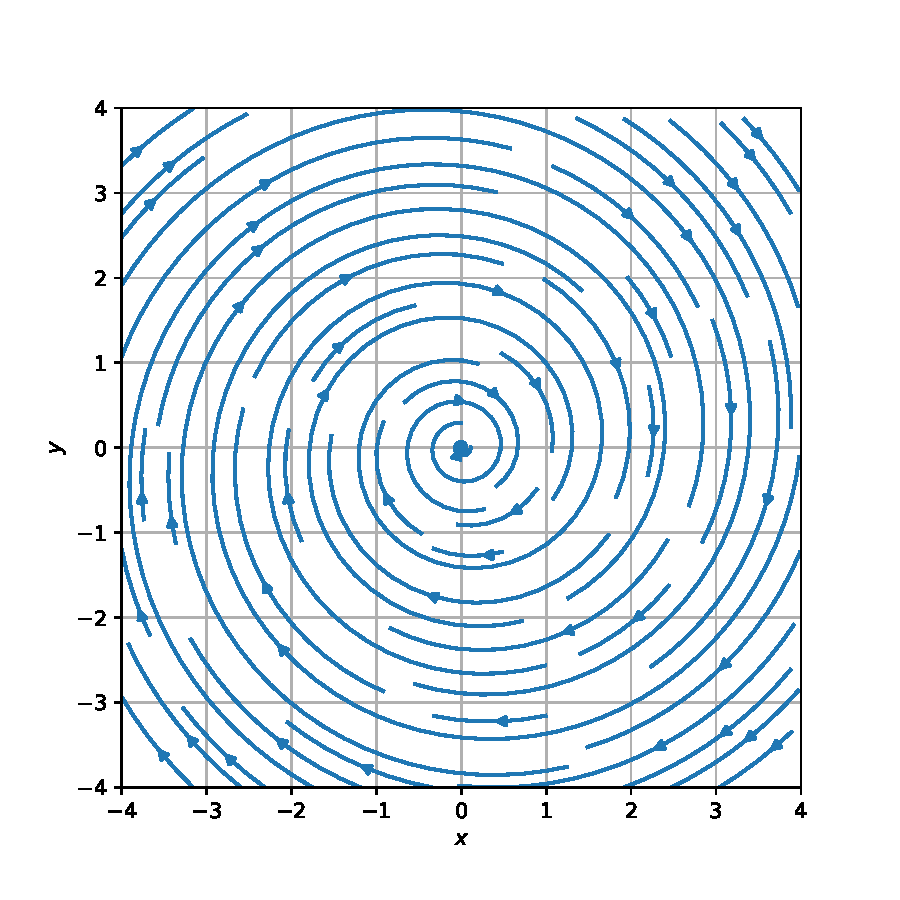
\includegraphics[scale=0.8]{2a1_0}
	\caption{Фазовый портрет в канонических координатах}
	\label{im:1a1_0}
\end{figure}



(iv) Изобразить фазовый портрет системы в исходных координатах.

\begin{figure}[H]
	\centering
	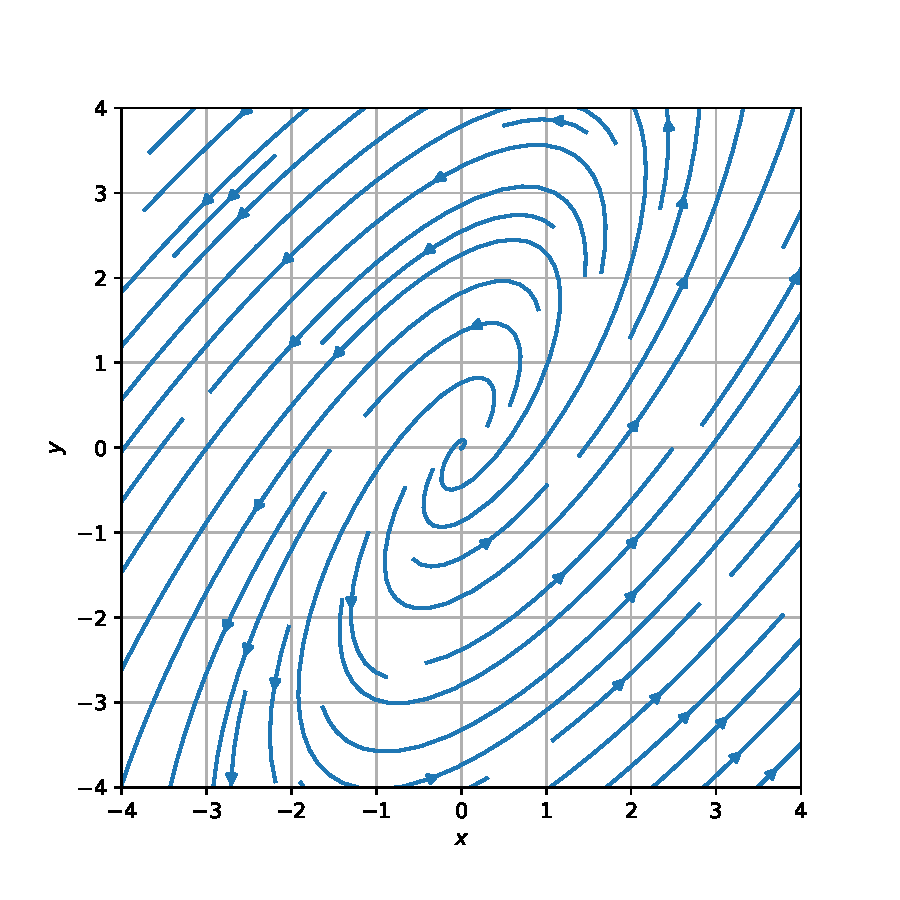
\includegraphics[scale=0.8]{2a1_1}
	\caption{Фазовый портрет в исходных координатах}
	\label{im:2a1_1}
\end{figure}

(v) Характер стационарной точки: $\lambda_{1,2}$ комплексны с ненулевой действительной частью, картина -- \textbf{неустойчивый фокус}.

	\subsection {Задача 2}
 Решить систему дифференциальных уравнений (Задача Коши): 
\begin{equation}
\left\{
\begin{array}{lr}
\dot{x} = -x+4y+3\cos{t}\\
\dot{y} = -x+3y
\end{array}
\right.
, \;\;\;\; x(\cdot)\in \textbf{R},\; y(\cdot)\in \textbf{R}
\label{eq:9}
\end{equation}

\textbf{Решение:} \par


(i) Найти общее решение соответствующей однородной системы.\\
Общее решение однородной системы совпадает с решением задачи 2 варианта IA. Приведем здесь только ответ:
\[\left(
\begin{array}{c}
x(t)\\
y(t)
\end{array}
\right)=e^{At}\left(
\begin{array}{c}
C_1 \\
C_2
\end{array}
\right)=Se^{\Lambda}S^{-1}\left(
\begin{array}{c}
C_1 \\
C_2
\end{array}
\right)=e^t
\left(
\begin{array}{cc}
2 & -1 \\
1 & 0
\end{array}
\right)
\left(
\begin{array}{cc}
1 & t \\
0 & 1
\end{array}
\right)
\left(
\begin{array}{cc}
0 & 1 \\
1- & 2
\end{array}
\right)\left(
\begin{array}{c}
C_1 \\
C_2
\end{array}
\right)=\]\[
=e^t
\left(
\begin{array}{cc}
1-2t & 4t \\
-t & 1+2t
\end{array}
\right)\left(
\begin{array}{c}
C_1 \\
C_2
\end{array}
\right)\]

Частное решение будем искать методом неопределенных коэффициентов:
\[x(t)_{\text{частн}}=a\cos{t}+b\sin{t}\]
\[y(t)_{\text{частн}}=c\cos{t}+d\sin{t}\]
Подставляя эти выражения в систему (\ref{eq:9}), получим:

\[
\left\{
\begin{array}{lr}
a = - \frac 3 2 \\
c = 0 \\
d =  \frac 3 2  \\
b= \frac 9 2 
\end{array}
\right.
\]
Общее решение уравнения есть сумма частного и однородного:

\begin{equation}
x(t) = e^t\left(\left(1-2t\right)C_1+4tC_2\right)- \frac 3 2 (\cos{t}-3\sin{t})
\label{eq:10}
\end{equation}
\begin{equation}
y(t) = e^t\left(-tC_1+\left(2t+1\right)C_2\right)+ \frac 3 2 \sin{t}
\label{eq:11}
\end{equation}

(ii) Найти траекторию системы (\ref{eq:9}), проходящую через начало координат.\\
Подставляя точку $(0;0;0)$ в (\ref{eq:10}) и (\ref{eq:11}), находим константы $C_1$ и $C_2$:

\[C_1 =3/2\;\;\;\;\; C_2 = 0\]

\[
x_0(t) = \frac 3 2 ( e^t\left(1-2t\right)-  \cos{t}+3\sin{t})\]\[
y_0(t) = - \frac 3 2 te^t+ \frac 3 2 \sin{t}
\]

(iii) Для траектории, найденной в (ii), найти пределы $\lim_{t\rightarrow\pm\infty}y(t)/x(t)$ (если они существуют).


\[\lim_{t\rightarrow+\infty}\frac{- \frac 3 2 te^t+ \frac 3 2 \sin{t}}{\frac 3 2 ( e^t\left(1-2t\right)-  \cos{t}+3\sin{t})}= \lim_{t\rightarrow+\infty}\frac{-3/2t}{-3/2 *2t}=\frac 1 2 \]

\[\lim_{t\rightarrow-\infty}\frac{- \frac 3 2 te^t+ \frac 3 2 \sin{t}}{\frac 3 2 ( e^t\left(1-2t\right)-  \cos{t}+3\sin{t})}=\lim_{t\rightarrow-\infty}\frac{ \frac 3 2 \sin{t}}{\frac 3 2 ( -  \cos{t}+3\sin{t})} \textbf{--  предела нет.}\]


	\subsection {Задача 3}
Для дифференциального уравнения 
\begin{equation}
y''+4y'+4y=\frac{e^{-2x}}{2x^2}, \;\;\;\; y(\cdot)\in \textbf{R},\; x>0
\label{eq:12}
\end{equation}

(i) Найти общее решение соотвествующего однородного уравнения.\\
Решение задачи аналогично решению задачи 3 варианта IA. Здесь корень характеристического уравнения имеет кратность 2. Решение:
\[y(x) = C_1e^{-2x}+C_2xe^{-2x}\]

(ii) Найти общее решение уравнения (\ref{eq:12}).\\
Будем решать уравнение методом вариации постоянной:

\[y(x)= C_1(x)e^{-2x}+C_2(x)xe^{-2x}\]
Получим систему:
\[ \left(
\begin{array}{cc}
e^{-2x} & xe^{-2x} \\
-2e^{-2x} & e^{-2x}(1-2x)
\end{array}
\right) \left(
\begin{array}{c}
C_1' \\
C_2'
\end{array} 
\right)= \left(
\begin{array}{c}
0 \\
e^{-2x}/2x^2
\end{array}
\right) \]
Найдем коэффициенты методом Крамера:
\[C_1' = -\frac 1 {2x}\]

\[C_2' = \frac 1  {2x^2}\]
Тогда общее решение:
\[y(x) = C_1e^{-2x}+C_2xe^{-2x}-\frac 1 2 e^{-2x}\ln(x)\]


	\subsection {Задача 4}

Для дифференциального уравнения
\begin{equation}
\ddot{x}-2\dot{x}+3x=e^{-t}\cos{t}, \;\;\;\; x(\cdot)\in \textbf{R}, t>0
\label{eq:13}
\end{equation}

(i) найти общее решение соответствующего однородного уравнения.\\
Характеристическое уравнение для левой части (\ref{eq:6}):
\[a^2-2a+3=0\]
\[a_{1,2}=1 \pm i\sqrt{2}\]
Тогда общее решение однородного уравнения:
\begin{equation}
x(t) = C_1e^t\cos{\sqrt{2}t}+C_2e^t\sin{\sqrt{2}t}
\label{eq:7}
\end{equation}

(ii) найти общее решение уравнения (\ref{eq:6}).\\
Частное решение для этой правой части ищем в виде:
\[ x(t) = ae^{-t}\cos{t}+be^{-t}\sin{t}\]
Поставляя в (\ref{eq:13}), находим коэффициенты: 
\[
\left\{
\begin{array}{lr}
a =\frac 5 {41}
b = -  \frac 4 {41}
\end{array}
\right.
\]
Суммируя частное и однородное решения, получим ответ:

\[x(t) =  C_1e^t\cos{\sqrt{2}t}+C_2e^t\sin{\sqrt{2}t}+\frac {5} {41} e^{-t}\cos{t}-\frac {4}{41}e^{-t}\sin{t} \]


	\section{Вариант IIIA}
		\subsection {Задача 1}


 Решить систему дифференциальных уравнений (Задача Коши): 
\begin{equation}
\left\{
\begin{array}{lr}
\dot{x} = x-y\\
\dot{y} = 5x-y
\end{array}
\right.
, \;\;\;\; x(\cdot)\in \textbf{R},\; y(\cdot)\in \textbf{R}
\label{eq:14}
\end{equation}

\textbf{Решение:} \par
Решение задачи полностью аналогично решению задачи 1 варианта IA.  

(i) Стационарные точки:

\[
\left\{
\begin{array}{lr}
\dot{x} = 0\\
\dot{y} = 0
\end{array}
\right.
\Leftrightarrow (0;0)
\]


(ii) Найдем собственные числа матрицы:
\[\lambda_{1,2}=\pm2i\]
\\Найдем собственные векторы:
\[\lambda_1:\;\;\;\;\; p^1=
\left(
\begin{array}{cc}
1+2i\\
5\\
\end{array}
\right)  
\]



\[\lambda_2:\;\;\;\; p^2=
\left(
\begin{array}{cc}
1-2i\\
5\\
\end{array}
\right) 
\]


 Каноническое преобразование координат:

\[
S = (u, \;-v) = \left(
\begin{array}{cc}
1 & -2\\
5 & 0\\
\end{array}
\right)\;\;\;\;\;
S^{-1} = \left(
\begin{array}{cc}
0 & 1/5\\
-1/2 & 1/10\\
\end{array}\right)\;\;\;\;\;
\Lambda = \left(
\begin{array}{cc}
0 & -2\\
2 & 0\\
\end{array}\right)
\]
\begin{figure}[H]
	\centering
	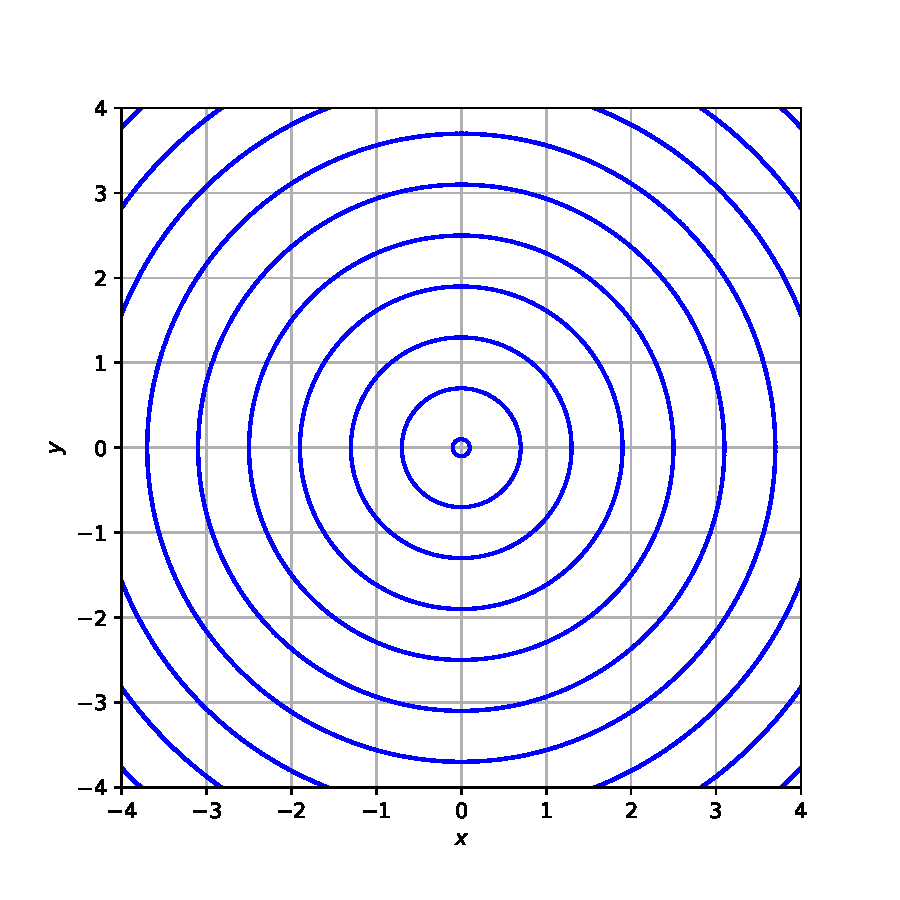
\includegraphics[scale=0.7]{3a1_0}
	\caption{Фазовый портрет в канонических координатах}
	\label{im:1a1_0}
\end{figure}
Система в новых координатах:
\[\left(
\begin{array}{c}
\dot{\alpha}_1\\
\dot{\alpha}_2
\end{array}
\right)=\Lambda\left(
\begin{array}{c}
{\alpha}_1 \\
{\alpha}_2
\end{array}
\right)\]

(iii) Прямые, при пересечении которых фазовые траектории параллельны осям $x$ и $y$.\\
Параллельно оси y:
\[\dot{x} = x-y=0\Leftrightarrow y = x\]\\
Параллельно оси x:
\[\dot{y} = 5x-y=0\Leftrightarrow y = 5x\]





(iv) Изобразить фазовый портрет системы в исходных координатах.

\begin{figure}[H]
	\centering
	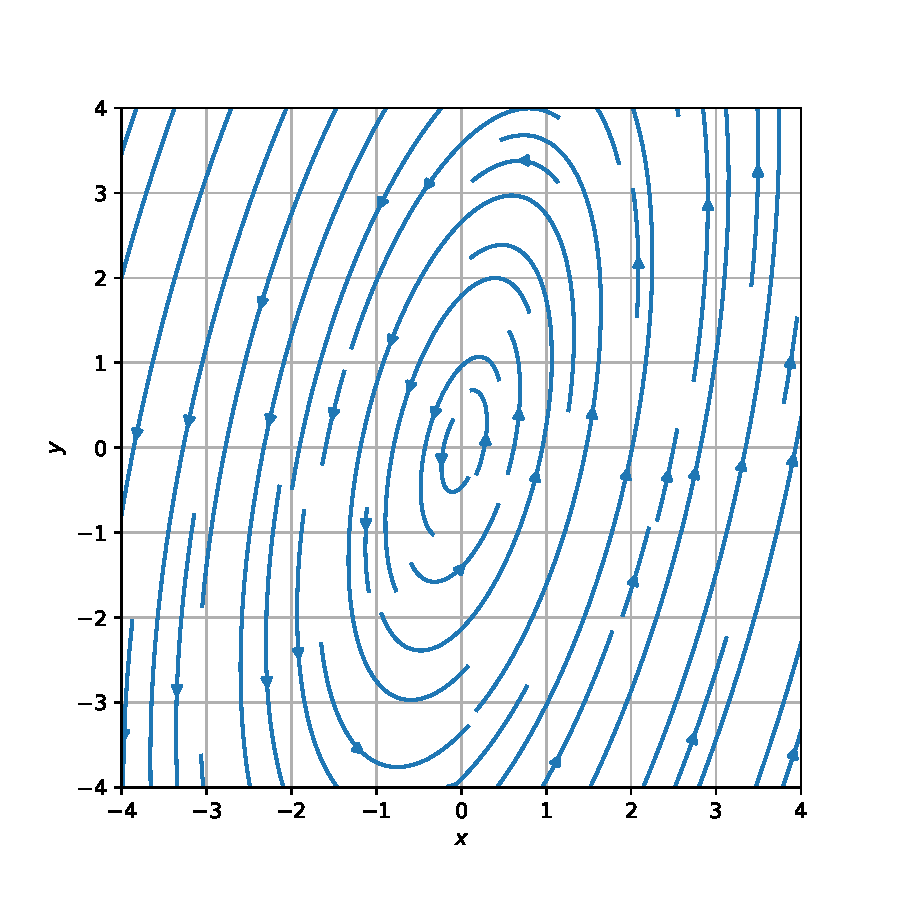
\includegraphics[scale=0.7]{3a1_1}
	\caption{Фазовый портрет в исходных координатах}
	\label{im:3a1_1}
\end{figure}
(v) Характер стационарной точки : $\lambda_{1,2}$ комплексны с нулевой действительной частью, картина -- \textbf{центр}.

	\subsection {Задача 2}
 Решить систему дифференциальных уравнений (Задача Коши): 
\begin{equation}
\left\{
\begin{array}{lr}
\dot{x} = x+2y+2e^{-t}\\
\dot{y} = 2x+y
\end{array}
\right.
, \;\;\;\; x(\cdot)\in \textbf{R},\; y(\cdot)\in \textbf{R}
\label{eq:16}
\end{equation}

\textbf{Решение:} \par


(i) Найти общее решение соответствующей однородной системы.\\
Собственные векторы и собственные значения для матрицы однородного уравнения:
\[\lambda_1 = 3:\;\;\;\;\; p^1=
\left(
\begin{array}{cc}
1\\
1\\
\end{array}
\right)  
\]

\[\lambda_2=-1\;\;\;\; p^2=
\left(
\begin{array}{cc}
-1\\
1\\
\end{array}
\right) 
\]
Общее решение:
\[\left(
\begin{array}{c}
x(t)\\
y(t)
\end{array}
\right)=C_1\left(
\begin{array}{c}
1 \\
1
\end{array}
\right)e^{3t}+C_2\left(
\begin{array}{c}
-1 \\
1
\end{array}
\right)e^{-t}\]
Частное решение будем искать методом вариации постоянной:
\[\left(
\begin{array}{c}
x(t)\\
y(t)
\end{array}
\right)=C_1(t)\left(
\begin{array}{c}
1 \\
1
\end{array}
\right)e^{3t}+C_2(t)\left(
\begin{array}{c}
-1 \\
1
\end{array}
\right)e^{-t}\]
Подставляя эти выражения в систему (\ref{eq:16}), получим:

\[
\left\{
\begin{array}{lr}
C_1  = t\\
C_2 = -\frac 1 4 e^{-4t}
\end{array}
\right.
\]
Общее решение уравнения есть сумма частного и однородного:

\begin{equation}
x(t) = C_1e^{-t}+C_2e^{3t}+e^{-t}(t-1/4)
\label{eq:17}
\end{equation}
\begin{equation}
y(t) = -e^{-t}C_1+C_2e^{3t}-e^{-t}(t+1/4)
\label{eq:18}
\end{equation}

(ii) Найти траекторию системы (\ref{eq:16}), проходящую через начало координат.\\
Подставляя точку $(0;0;0)$ в (\ref{eq:17}) и (\ref{eq:18}), находим константы $C_1$ и $C_2$:

\[C_1 = 0\;\;\;\;\; C_2 = 1/4\]

\[
x_0(t) =\frac 1 4 (e^{3t}+4e^{-t}t-e^{-t})\]\[
y_0(t) = 1/4e^{3t}-e^{-t}(t+1/4)
\]

(iii) Для траектории, найденной в (ii), найти пределы $\lim_{t\rightarrow\pm\infty}y(t)/x(t)$ (если они существуют).


\[\lim_{t\rightarrow+\infty}\frac{1/4e^{3t}-e^{-t}(t+1/4)}{\frac 1 4 (e^{3t}+4e^{-t}t-e^{-t})}=1 \]

\[\lim_{t\rightarrow-\infty}\frac{1/4e^{3t}-e^{-t}(t+1/4)}{\frac 1 4 (e^{3t}+4e^{-t}t-e^{-t})}=-1\]





	\subsection {Задача 3}
Для дифференциального уравнения 
\begin{equation}
y''+2y'+y=\frac{e^{-x}}{x}, \;\;\;\; y(\cdot)\in \textbf{R},\; x>0
\label{eq:19}
\end{equation}

(i) Найти общее решение соотвествующего однородного уравнения.\\
Решение задачи аналогично решению задачи 3 варианта IIA:
\[y(x) = C_1e^{-x}+C_2xe^{-x}\]

(ii) Найти общее решение уравнения (\ref{eq:19}).\\
Будем решать уравнение методом вариации постоянной:

\[y(x)= C_1(x)e^{-x}+C_2(x)xe^{-x}\]
Получим систему:
\[ \left(
\begin{array}{cc}
e^{-x} & xe^{-x} \\
-e^{-x} & e^{-x}(1-x)
\end{array}
\right) \left(
\begin{array}{c}
C_1' \\
C_2'
\end{array} 
\right)= \left(
\begin{array}{c}
0 \\
e^{-x}/x
\end{array}
\right) \]
Найдем коэффициенты методом Крамера:
\[C_1' = -1\]

\[C_2' = \frac 1  {x}\]
Тогда общее решение:
\[y(x) = C_1e^{-x}+C_2xe^{-x}+xe^{-x}\ln{x}\]


	\subsection {Задача 4}

Для дифференциального уравнения
\begin{equation}
\dddot{x}-\dot{x}=t\cos{t}, \;\;\;\; x(\cdot)\in \textbf{R}
\label{eq:20}
\end{equation}

(i) найти общее решение соответствующего однородного уравнения.\\
Характеристическое уравнение для левой части (\ref{eq:20}):
\[a^3-a=0\]
\[a_{1,2}=\pm1\]
\[a_0=0\]
Тогда общее решение однородного уравнения:
\begin{equation}
x(t) = C_1e^t+C_2e^{-t}+C_3
\label{eq:21}
\end{equation}

(ii) найти общее решение уравнения (\ref{eq:20}).\\
Частное решение для этой правой части ищем в виде:
\[ x(t) = a\cos{t}+bt\cos{t}+c\sin{t}+dt\sin{t}\]
Поставляя в (\ref{eq:20}), находим коэффициенты: 
\[
\left\{
\begin{array}{lr}
a =-1\\
b = 0\\
c = 0\\
d = -\frac 1 2
\end{array}
\right.
\]
Суммируя частное и однородное решения, получим ответ:

\[x(t) = -\cos{t}-\frac 1 2 t\sin{t}+C_1e^{-t}+C_2+C_3e^t \]











	\section{Вариант IB}
		\subsection {Задача 1}


 Решить систему дифференциальных уравнений (Задача Коши): 
\begin{equation}
\left\{
\begin{array}{lr}
\dot{x} = 3x+y\\
\dot{y} = -x+y
\end{array}
\right.
, \;\;\;\; x(\cdot)\in \textbf{R},\; y(\cdot)\in \textbf{R}
\label{eq:22}
\end{equation}

\textbf{Решение:} \par
Решение задачи полностью аналогично решению задачи 1 варианта IA.  

(i) Стационарные точки:

\[
\left\{
\begin{array}{lr}
\dot{x} = 0\\
\dot{y} = 0
\end{array}
\right.
\Leftrightarrow (0;0)
\]


(ii) Найти каноническое преобразование координат.
\[\lambda =2\;\;\text{-- собственное число кратности 2}\]
Собственный вектор:
\[p=
\left(
\begin{array}{cc}
-1\\
1\\
\end{array}
\right)
\]
Собственному числу соответствует одномерное пространство собственных векторов. Найдем присоединенный вектор:\\
\[(A-\lambda \hat{I})v=p\]
\[v=
\left(
\begin{array}{cc}
-1\\
0\\
\end{array}
\right)
\]
\[A = S\Lambda S^{-1}\]
\[
S = \left(
\begin{array}{cc}
-1 & -1\\
1 & 0\\
\end{array}
\right)\;\;\;\;\;
S^{-1} = \left(
\begin{array}{cc}
0 & 1\\
-1 & -1\\
\end{array}\right)\;\;\;\;\;
\Lambda = \left(
\begin{array}{cc}
2 & 1\\
0 & 2\\
\end{array}\right)
\]
Система в новых координатах:
\[\left(
\begin{array}{c}
\dot{\alpha}_1\\
\dot{\alpha}_2
\end{array}
\right)=\Lambda\left(
\begin{array}{c}
{\alpha}_1 \\
{\alpha}_2
\end{array}
\right)\]
\begin{figure}[H]
	\centering
	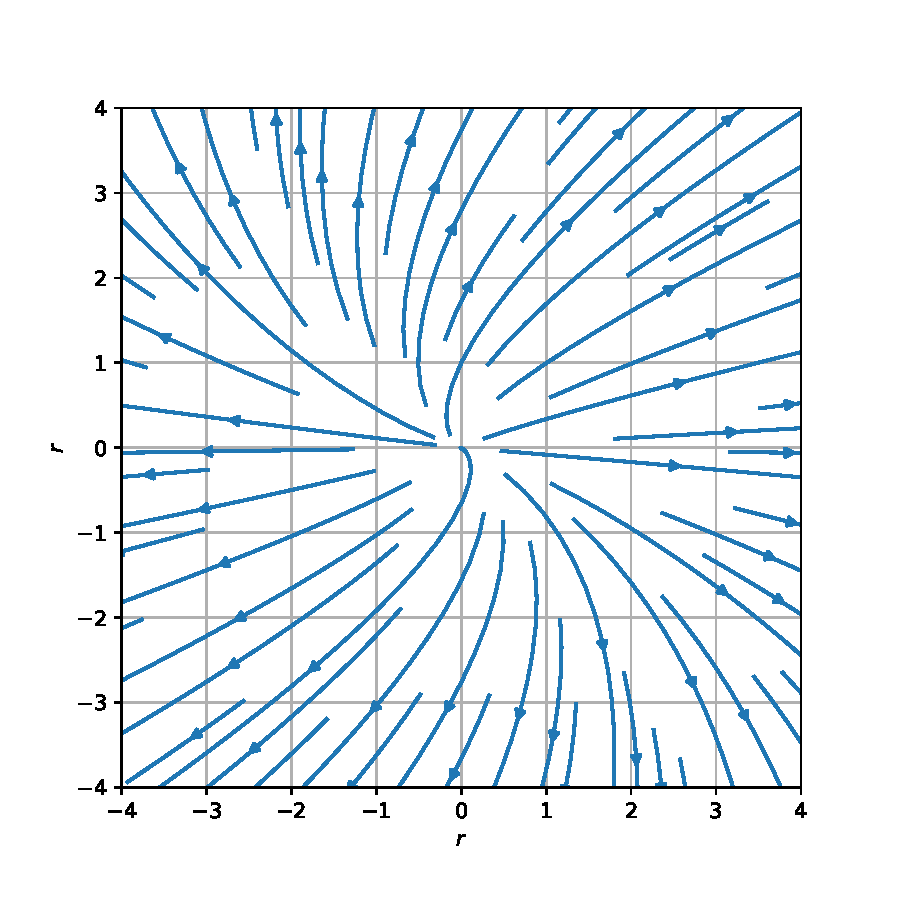
\includegraphics[scale=0.8]{1b1_0}
	\caption{Фазовый портрет в этих координатах}
	\label{im:1b1_0}
\end{figure}


(iii) Прямые, при пересечении которых фазовые траектории параллельны осям $x$ и $y$.\\
Параллельно оси y:
\[\dot{x} = 3x+y=0\Leftrightarrow y = -3x\]\\
Параллельно оси x:
\[\dot{y} = -x+y=0\Leftrightarrow y = x\]

(iv) Изобразить фазовый портрет системы в исходных координатах.

\begin{figure}[H]
	\centering
	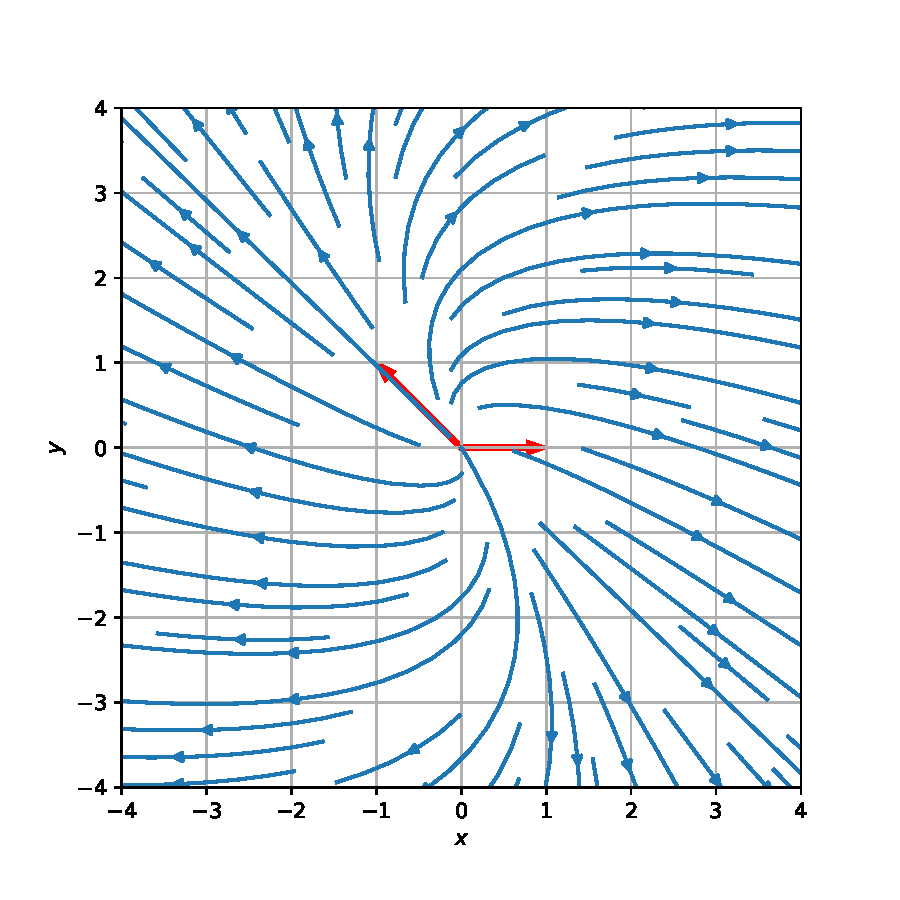
\includegraphics[scale=0.8]{1b1_1}
	\caption{Фазовый портрет в исходных координатах}
	\label{im:1b1_1}
\end{figure}
(v) Характер стационарной точки: $\lambda_{1,2}>0 \Rightarrow$ стационарная точка -- \textbf{неустойчивый вырожденный узел}.

	\subsection {Задача 2}
 Решить систему дифференциальных уравнений (Задача Коши): 
\begin{equation}
\left\{
\begin{array}{lr}
\dot{x} = -x+4y+e^{-t}\\
\dot{y} = 2x+y+1
\end{array}
\right.
, \;\;\;\; x(\cdot)\in \textbf{R},\; y(\cdot)\in \textbf{R}
\label{eq:23}
\end{equation}

\textbf{Решение:} \par


(i) Найти общее решение соответствующей однородной системы.\\

Собственные векторы и собственные значения для матрицы однородного уравнения:
\[\lambda_1 = -3:\;\;\;\;\; p^1=
\left(
\begin{array}{cc}
-2\\
1\\
\end{array}
\right)  
\]



\[\lambda_2=3\;\;\;\; p^2=
\left(
\begin{array}{cc}
1\\
1\\
\end{array}
\right) 
\]

Общее решение:
\[\left(
\begin{array}{c}
x(t)\\
y(t)
\end{array}
\right)=C_1\left(
\begin{array}{c}
-2 \\
1
\end{array}
\right)e^{-3t}+C_2\left(
\begin{array}{c}
1 \\
1
\end{array}
\right)e^{3t}\]

Частное решение будем искать методом вариации постоянной:
\[x(t)_{\text{частн}}=a+be^{-t}\]
\[y(t)_{\text{частн}}=c+de^{-t}\]
Подставляя эти выражения в систему (\ref{eq:23}), получим:

\[
\left\{
\begin{array}{lr}
a = -\frac {4} {9}\\
b = \frac {1} {4}\\
c = -\frac {1} {9}\\
d = -\frac {1} {4}\\
\end{array}
\right.
\]
Общее решение уравнения есть сумма частного и однородного:

\begin{equation}
x(t) = -2C_1e^{-3t}+C_2e^{3t}-\frac 4 9 + \frac 1 4 e^{-t}
\label{eq:24}
\end{equation}
\begin{equation}
y(t) =C_1e^{-3t}+C_2e^{3t}- \frac 1 9 -\frac 1 4 e^{-t}
\label{eq:25}
\end{equation}

(ii) Найти траекторию системы (\ref{eq:23}), проходящую через начало координат.\\
Подставляя точку $(0;0;0)$ в (\ref{eq:24}) и (\ref{eq:24}), находим константы $C_1$ и $C_2$:

\[C_1 = \frac 1 {18}\;\;\;\;\; C_2 = \frac{11} {36}\]

\[
x_0(t) =-\frac 1 9 e^{-3t}+\frac{11}{36}e^{3t}-\frac 4 9 + \frac 1 4 e^{-t}\]
\[
y_0(t) =\frac 1 {18}e^{-3t}+\frac{11} {36} e^{3t}- \frac 1 9 -\frac 1 4 e^{-t}
\]

(iii) Для траектории, найденной в (ii), найти пределы $\lim_{t\rightarrow\pm\infty}y(t)/x(t)$ (если они существуют).


\[\lim_{t\rightarrow+\infty}\frac{\frac 1 {18}e^{-3t}+\frac{11} {36} e^{3t}- \frac 1 9 -\frac 1 4 e^{-t}}{-\frac 1 9 e^{-3t}+\frac{11}{36}e^{3t}-\frac 4 9 + \frac 1 4 e^{-t}}= 1\]

\[\lim_{t\rightarrow-\infty}\frac{\frac 1 {18}e^{-3t}+\frac{11} {36} e^{3t}- \frac 1 9 -\frac 1 4 e^{-t}}{-\frac 1 9 e^{-3t}+\frac{11}{36}e^{3t}-\frac 4 9 + \frac 1 4 e^{-t}}=-\frac 1 2\]





	\subsection {Задача 3}
Для дифференциального уравнения 
\begin{equation}
y''+4y=\frac{1}{\cos{2x}}, \;\;\;\; y(\cdot)\in \textbf{R},\; x>0
\label{eq:26}
\end{equation}

(i) Найти общее решение соотвествующего однородного уравнения.\\
\textit{См. задачу 3 вариант IA (уравнение (\ref{eq:19}))}\\
\[y(x) =C_2\cos{2x}+C_1\sin{2x}\]


(ii) Найти общее решение уравнения (\ref{eq:26}).\\
Будем решать уравнение методом вариации постоянной:

\[y(x)= C_1(t)\cos{2x}+C_2(t)\sin{2x}\]
Получим систему:
\[ \left(
\begin{array}{cc}
\sin{2x} & \cos{2x} \\
2\cos{2x} & -2\sin{2x}
\end{array}
\right) \left(
\begin{array}{c}
C_1' \\
C_2'
\end{array} 
\right)= \left(
\begin{array}{c}
0 \\
\frac{1}{\cos{2x}}
\end{array}
\right) \]
Найдем коэффициенты методом Крамера:
\[C_1' = \frac{\begin{vmatrix}
0 & \cos{2x} \\
\frac{1}{\cos{2x}} & -2\sin{2x}
\end{vmatrix}}{\begin{vmatrix}
\sin{2x} & \cos{2x} \\
2\cos{2x} & -2\sin{2x}
\end{vmatrix}}= -1/2\]

\[C_2' = \frac{\begin{vmatrix}
\sin{2x} & 0 \\
2\cos{2x} & \frac{1}{\cos{2x}}
\end{vmatrix}}{\begin{vmatrix}
\sin{2x} & \cos{2x} \\
2\cos{2x} & -2\sin{2x}
\end{vmatrix}}= -\tg{2x}/2\]
Находим 
\[C_1 = -1/2x\]
\[C_2=1/4\ln{|\cos{(2x)}|}\]
Тогда общее решение:
\[y(x) = C_1\sin{2x}+C_2\cos{2x}+\frac {1} {2} x\sin{2x}+\frac 1 4 \ln{|\cos{(2x)}|}\cos{2x}\]





	\subsection {Задача 4}

Для дифференциального уравнения
\begin{equation}
x^{(iv)}-16x=80e^{2t}\sin{2t}, \;\;\;\; x(\cdot)\in \textbf{R}, t> 0
\label{eq:27}
\end{equation}

(i) найти общее решение соответствующего однородного уравнения.\\
Характеристическое уравнение для левой части (\ref{eq:27}):
\[a^4-16=0\]
\[a_1 = 2,\;\;a_2 =-2,\;\;a_3=2i,\;\;a_4=-2i\]
Тогда общее решение однородного уравнения:
\begin{equation}
x(t) = C_1e^{2t}+C_2\cos{2t}+C_3\sin{2t}+C_4e^{-2t}
\label{eq:28}
\end{equation}

(ii) найти общее решение уравнения (\ref{eq:27}).\\
Частное решение для этой правой части ищем в виде:
\[ x(t) = ae^{2t}\cos{2t}+be^{2t}\sin{2t}\]
Подставляя в (\ref{eq:27}), находим коэффициенты: 
\[
\left\{
\begin{array}{lr}
a =0\\
b = -1
\end{array}
\right.
\]
Суммируя частное и однородное решения, получим ответ:

\[x(t) = C_1e^{2t}+C_2\cos{2t}+C_3\sin{2t}+C_4e^{-2t}-e^{2t}\sin{2t} \]

















	\section{Вариант IIB}
		\subsection {Задача 1}


 Решить систему дифференциальных уравнений (Задача Коши): 
\begin{equation}
\left\{
\begin{array}{lr}
\dot{x} = -x-y\\
\dot{y} = -y/4
\end{array}
\right.
, \;\;\;\; x(\cdot)\in \textbf{R},\; y(\cdot)\in \textbf{R}
\label{eq:29}
\end{equation}

\textbf{Решение:} \par
Решение задачи полностью аналогично решению задачи 1 варианта IA.  

(i) Стационарные точки:

\[
\left\{
\begin{array}{lr}
\dot{x} = 0\\
\dot{y} = 0
\end{array}
\right.
\Leftrightarrow (0;0)
\]


(ii) Найдем собственные числа и векторы матрицы:

\[\lambda_1 = -1\;\;\;\;\; p^1=
\left(
\begin{array}{cc}
1\\
0\\
\end{array}
\right)  
\]
\[\lambda_2=-1/4\;\;\;\; p^2=
\left(
\begin{array}{cc}
-4/3\\
1\\
\end{array}
\right) 
\]


Каноническое преобразование координат:
\[A = S\Lambda S^{-1}\]
\[
S = \left(
\begin{array}{cc}
1 & -4/3\\
0 & 1\\
\end{array}
\right)\;\;\;\;\;
S^{-1} = \left(
\begin{array}{cc}
1 & 4/3\\
0 & 1\\
\end{array}\right)\;\;\;\;\;
\Lambda = \left(
\begin{array}{cc}
-1 & 0\\
0 & -1/4\\
\end{array}\right)
\]
\begin{figure}[H]
	\centering
	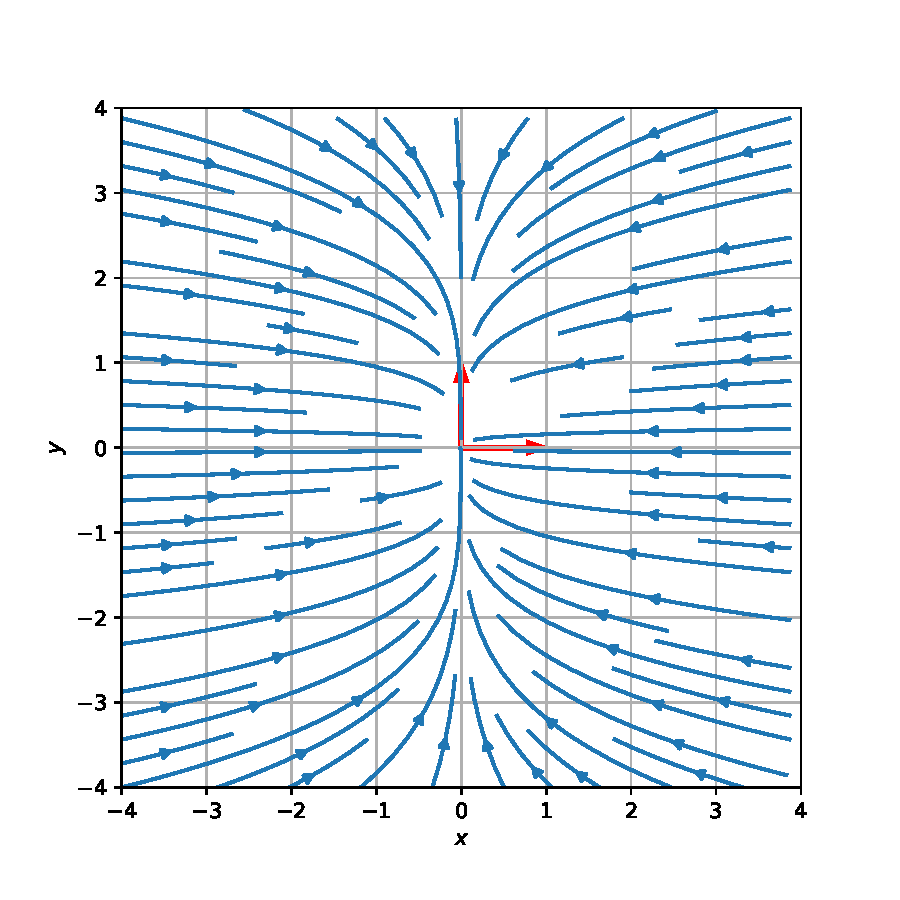
\includegraphics[scale=0.7]{2b1_0}
	\caption{Фазовый портрет в канонических координатах}
	\label{im:1b1_0}
\end{figure}
Система в новых координатах:
\[\left(
\begin{array}{c}
\dot{\alpha}_1\\
\dot{\alpha}_2
\end{array}
\right)=\Lambda\left(
\begin{array}{c}
{\alpha}_1 \\
{\alpha}_2
\end{array}
\right)\]
 


(iii) Прямые, при пересечении которых фазовые траектории параллельны осям $x$ и $y$.\\
Параллельно оси y:
\[\dot{x} = -x-y=0\Leftrightarrow y = -x\]\\
Параллельно оси x:
\[\dot{y} = -y/4=0\Leftrightarrow y = 0\]




(iv) Изобразить фазовый портрет системы в исходных координатах.

\begin{figure}[H]
	\centering
	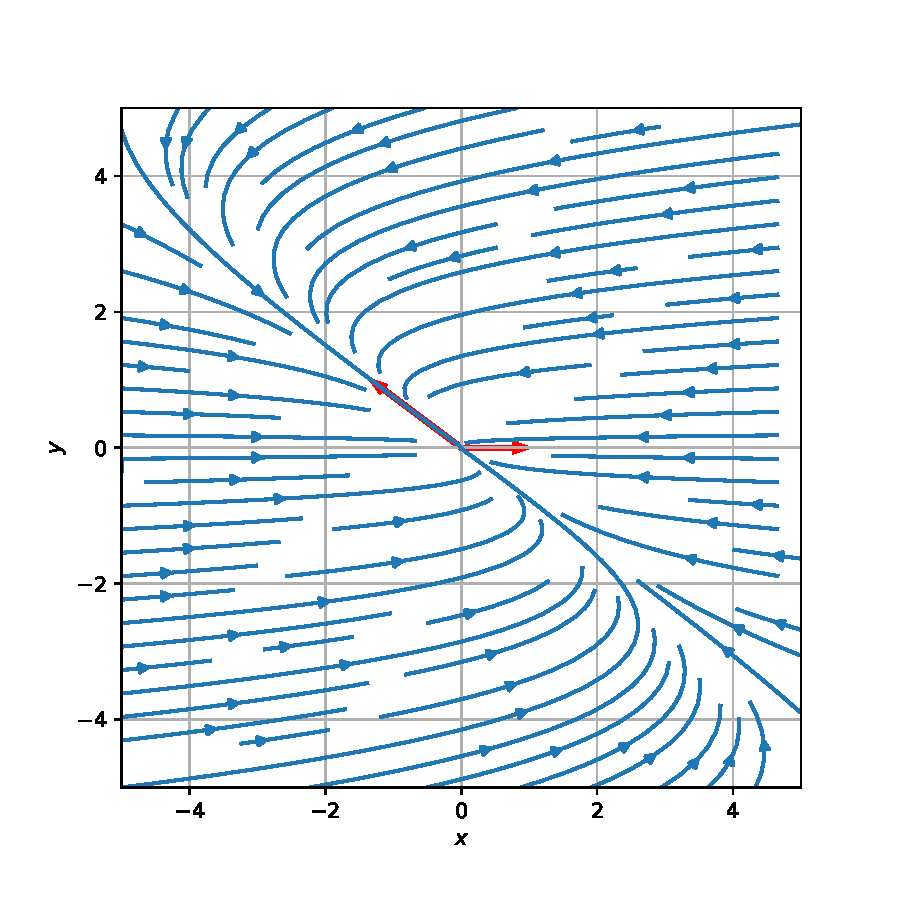
\includegraphics[scale=0.7]{2b1_1}
	\caption{Фазовый портрет в исходных координатах}
	\label{im:1b1_1}
\end{figure}

(v) Характер стационарной точки: $\lambda_{1,2}$ одного знака и различны, картина -- \textbf{устойчивый узел}.

	\subsection {Задача 2}
 Решить систему дифференциальных уравнений (Задача Коши): 
\begin{equation}
\left\{
\begin{array}{lr}
\dot{x} = -x+4y+\sin{t}\\
\dot{y} = 2x-y
\end{array}
\right.
, \;\;\;\; x(\cdot)\in \textbf{R},\; y(\cdot)\in \textbf{R}
\label{eq:30}
\end{equation}

\textbf{Решение:} \par


(i) Найти общее решение соответствующей однородной системы.\\

Собственные векторы и собственные значения для матрицы однородного уравнения:
\[\lambda_1 = -1-2\sqrt 2 :\;\;\;\;\; p^1=
\left(
\begin{array}{cc}
-\sqrt 2\\
1\\
\end{array}
\right)  
\]



\[\lambda_2=2\sqrt 2-1\;\;\;\; p^2=
\left(
\begin{array}{cc}
\sqrt 2\\
1\\
\end{array}
\right) 
\]

Общее решение:
\[\left(
\begin{array}{c}
x(t)\\
y(t)
\end{array}
\right)=C_1\left(
\begin{array}{c}
-\sqrt 2 \\
1
\end{array}
\right)e^{(-1-2\sqrt 2)t}+C_2\left(
\begin{array}{c}
\sqrt 2 \\
1
\end{array}
\right)e^{(2\sqrt 2-1)t}\]

Частное решение будем искать методом вариации постоянной:
\[x(t)_{\text{частн}}=a\cos{t}+b\sin{t}\]
\[y(t)_{\text{частн}}=c\cos{t}+d\sin{t}\]
Подставляя эти выражения в систему (\ref{eq:30}), получим:

\[
\left\{
\begin{array}{lr}
a = -\frac {5} {34}\\
b = -\frac {3} {34}\\
c = -\frac {1} {17}\\
d = -\frac {4} {17}\\
\end{array}
\right.
\]
Общее решение уравнения есть сумма частного и однородного:

\begin{equation}
x(t) = -C_1\sqrt 2 e^{(-1-2\sqrt 2)t}+C_2\sqrt 2 e^{(-1+2\sqrt 2)t} -\frac {5} {34}\cos{t}-\frac {3} {34}\sin{t}
\label{eq:31}
\end{equation}
\begin{equation}
y(t) =C_1 e^{(-1-2\sqrt 2)t}+C_2 e^{(-1+2\sqrt 2)t} -\frac {1} {17}\cos{t}-\frac {4} {17}\sin{t}
\label{eq:32}
\end{equation}

(ii) Найти траекторию системы (\ref{eq:30}), проходящую через начало координат.\\
Подставляя точку $(0;0;0)$ в (\ref{eq:31}) и (\ref{eq:32}), находим константы $C_1$ и $C_2$:

\[C_1 = \frac{5\sqrt{2}-4}{136}\;\;\;\;\; C_2 = \frac{12- 5\sqrt{2}}{136}\]

\[
x_0(t) = -\frac{5-2\sqrt{2}}{68} e^{(-1-2\sqrt 2)t}+\frac{6\sqrt{2}- 5}{68} e^{(-1+2\sqrt 2)t} -\frac {5} {34}\cos{t}-\frac {3} {34}\sin{t}
\]\[
y_0(t) = \frac{5\sqrt{2}-4}{136} e^{(-1-2\sqrt 2)t}+\frac{12- 5\sqrt{2}}{136}e^{(-1+2\sqrt 2)t} -\frac {1} {17}\cos{t}-\frac {4} {17}\sin{t}
\]

(iii) Для траектории, найденной в (ii), найти пределы $\lim_{t\rightarrow\pm\infty}y(t)/x(t)$ (если они существуют).


\[\lim_{t\rightarrow+\infty}\frac{\frac{5\sqrt{2}-4}{136} e^{(-1-2\sqrt 2)t}+\frac{12- 5\sqrt{2}}{136}e^{(-1+2\sqrt 2)t} -\frac {1} {17}\cos{t}-\frac {4} {17}\sin{t}}{-\frac{5-2\sqrt{2}}{68} e^{(-1-2\sqrt 2)t}+\frac{6\sqrt{2}- 5}{68} e^{(-1+2\sqrt 2)t} -\frac {5} {34}\cos{t}-\frac {3} {34}\sin{t}}=1 \]

\[\lim_{t\rightarrow-\infty}\frac{\frac{5\sqrt{2}-4}{136} e^{(-1-2\sqrt 2)t}+\frac{12- 5\sqrt{2}}{136}e^{(-1+2\sqrt 2)t} -\frac {1} {17}\cos{t}-\frac {4} {17}\sin{t}}{-\frac{5-2\sqrt{2}}{68} e^{(-1-2\sqrt 2)t}+\frac{6\sqrt{2}- 5}{68} e^{(-1+2\sqrt 2)t} -\frac {5} {34}\cos{t}-\frac {3} {34}\sin{t}}=+\infty\]





	\subsection {Задача 3}
Для дифференциального уравнения 
\begin{equation}
y''+2y'+y=\frac{e^{-x}}{x}, \;\;\;\; y(\cdot)\in \textbf{R},\; x>0
\label{eq:33}
\end{equation}

(i) Найти общее решение соотвествующего однородного уравнения.

(ii) Найти общее решение уравнения (\ref{eq:33}).\\
\textit{См. задачу 3 вариант IIIA (уравнение (\ref{eq:19}))}


	\subsection {Задача 4}

Для дифференциального уравнения
\begin{equation}
\dddot{x}-4\ddot{x}+5\dot{x}-2x=2t+3, \;\;\;\; x(\cdot)\in \textbf{R}, t>0
\label{eq:34}
\end{equation}

(i) найти общее решение соответствующего однородного уравнения.\\
Характеристическое уравнение для левой части (\ref{eq:34}):
\[a^3-4a^2+5a-2=0\]
\[(a-2)(a-1)^2=0\]
\[a_{1,2}=1\;\;\;\\;a_3=2\]
Тогда общее решение однородного уравнения:
\begin{equation}
x(t) = C_1e^t+C_2te^{t}+C_3e^{2t}
\label{eq:35}
\end{equation}

(ii) найти общее решение уравнения (\ref{eq:34}).\\
Частное решение для этой правой части ищем в виде:
\[ x(t) = a+bt\]
Подставляя в (\ref{eq:34}), находим коэффициенты: 
\[
\left\{
\begin{array}{lr}
a =-4\\
b = -1
\end{array}
\right.
\]
Суммируя частное и однородное решения, получим ответ:

\[x(t) = C_1e^t+C_2te^{t}+C_3e^{2t}-t-4 \]






\end{document}